% vim:spelllang=ru,en
\documentclass[a4paper,12pt,notitlepage,headsepline,pdftex]{scrartcl}

\usepackage{cmap} % чтобы работал поиск по PDF
\usepackage[T2A]{fontenc}
\usepackage[utf8]{inputenc}
\usepackage[english,russian]{babel}
\usepackage{concrete}
\usepackage{cite}
\usepackage{url}

\usepackage{textcase}
\usepackage[pdftex]{graphicx}

\usepackage{lscape}

\pdfcompresslevel=9 % сжимать PDF
\usepackage{pdflscape} % для возможности альбомного размещения некоторых страниц
\usepackage[pdftex]{hyperref}
% настройка ссылок в оглавлении для pdf формата
\hypersetup{unicode=true,
            pdftitle={ПОЭВМ Лаба №1},
            pdfauthor={Погода Михаил},
            pdfcreator={pdflatex},
            pdfsubject={},
            pdfborder    = {0 0 0},
            bookmarksopen,
            bookmarksnumbered,
            bookmarksopenlevel = 2,
            pdfkeywords={},
            colorlinks=true, % установка цвета ссылок в оглавлении
            citecolor=black,
            filecolor=black,
            linkcolor=black,
            urlcolor=blue}

\usepackage{amsmath}
\usepackage{amssymb}
\usepackage{moreverb}
\usepackage{indentfirst}
\usepackage{misccorr}

\usepackage{xtab}
\usepackage{nccfoots}
\usepackage{listings}

\lstloadlanguages{C++}
\lstset{language=C++,basicstyle=\scriptsize,frame=tb,commentstyle=\itshape,stringstyle=\bfseries,extendedchars=false}
\begin{document}
\begin{titlepage}
  \begin{center}
    \large
    \MakeUppercase{Министерство образования и науки,}

    \MakeUppercase{молодёжи и спорта Украины}

    \mbox{\MakeUppercase{Национальный технический университет Украины}}

    \MakeUppercase{,,Киевский политехнический институт''}

    \addvspace{6pt}

    \normalsize
    Кафедра прикладной математики

    \vfill

    \textbf{Отчёт}

    Лабораторная работа №1

    по дисциплине ,,Программное обеспечение ЭВМ''

    \emph{,,Решение систем линейных уравнений''}
  \end{center}

  \vfill

  \noindent
  \begin{minipage}{0.3\textwidth}
    Выполнил

    студент группы КМ-92

    Погода~М.\,В.
  \end{minipage}
  \hfill
  \begin{minipage}{0.4\textwidth}
    Проверила:

    Ковальчук"=Химюк~Л.\,А.
  \end{minipage}
  \vfill

  \begin{center}
    КИЕВ

    2012
  \end{center}
\end{titlepage}
\tableofcontents
\newpage
\section{Постановка задачи}
  Дана матрица коэффициентов $A$ и столбец свободных членов $b$.
  Необходимо:
  \begin{itemize}
    \item Решить на ЭВМ данную СЛАУ\footnote{Система линейный алгебраических
      уравнений}.
    \item Оценить точность решения.
  \end{itemize}
\section{Исходные данные}
  \hfill\emph{Вариант~11}

  Матрица коэффициентов:
  \begin{equation}
    A = \left(\begin{matrix}
          3.82 & 1.02 & 0.75 & 0.81\\
          1.05 & 4.53 & 0.98 & 1.53\\
          0.73 & 0.85 & 4.71 & 0.81\\
          0.88 & 0.81 & 1.28 & 3.50\end{matrix}\right)
    \label{eq:A}
  \end{equation}

  \begin{equation}
    b = \left( \begin{matrix}
      15.655\\
      22.705\\
      23.480\\
      16.110
    \end{matrix}\right)
    \label{eq:b}
  \end{equation}

  Метод решения --- \emph{метод Жордана"=Гаусса}.
\newpage
\section{Теоретические сведения}
  Метод Жордана"=Гаусса, или метод полного исключения неизвестных, имеет
  следующий алгоритм:

  \begin{enumerate}
    \item Выбирают первый слева столбец матрицы, в котором есть хоть одно
      отличное от нуля значение.
    \item Если самое верхнее число в этом столбце есть ноль, то меняют всю
      первую строку матрицы с другой строкой матрицы, где в этой колонке нет
      нуля.
    \item Все элементы первой строки делят на верхний элемент выбранного
      столбца.
    \item Из оставшихся строк вычитают первую строку, умноженную на первый
      элемент соответствующей строки, с целью получить первым элементом каждой
      строки (кроме первой) ноль.
    \item Далее проводят такую же процедуру с матрицей, получающейся из
      исходной матрицы после вычёркивания первой строки и первого столбца.
    \item После повторения этой процедуры  раз получают верхнюю треугольную
      матрицу.
    \item Вычитают из предпоследней строки последнюю строку, умноженную на
      соответствующий коэффициент, с тем, чтобы в предпоследней строке
      осталась только 1 на главной диагонали.
    \item Повторяют предыдущий шаг для последующих строк.
      В итоге получают единичную матрицу и решение на месте свободного вектора
      (с ним необходимо проводить все те же преобразования).
  \end{enumerate}
\newpage
\section{Решение}
  \subsection{Решение СЛАР на ЭВМ}
    \begin{equation}
      x = \left( \begin{matrix}
        2.160\\
        3.028\\
        3.763\\
        1.983
      \end{matrix}\right)
      \label{eq:x}
    \end{equation}
  \subsection{Проверка полученного решения подстановкой}
    \begin{equation}
      b^* = \left( \begin{matrix}
        15.655\\
        22.707\\
        23.481\\
        16.111
      \end{matrix}\right)
      \label{eq:b_ast}
    \end{equation}
  \subsection{Погрешность решения}
    \begin{equation}
      \Delta b = \left( \begin{matrix}
        3.50\\
        1.57\\
        5.60\\
        6.20
      \end{matrix}\right) \cdot 10^{-4}
      \label{eq:delta}
    \end{equation}
\newpage
\section{Описание программы}
  Программа написана на языке C++ с использованием библиотек
  boost\footnote{\url{boost.org}} и Qt\footnote{\url{qt-project.org}}.

  Входными данными является файл, который выбирается путём диалога открытия
  файла, и имеющий следующую структуру:
  \begin{enumerate}
    \item Целое положительное число \verb'n', характеризующее количество
      уравнений в данной СЛАУ;
    \item $n \times (n+1)$ чисел с плавающей точкой, являющиеся коэффициентами
      присоединённой матрицы $\bar{A}$.
  \end{enumerate}

  Результатом работы программы есть присоединённая матрица $\bar{A^\prime}$
  после применения к ней метода Жордана"=Гаусса.

  Для отображения этих матриц программа использует
  \LaTeX{}\footnote{\url{latex-project.org}} и
  ImageMagick\footnote{\url{www.imagemagick.org}}.


  \begin{landscape}
    \begin{figure}[h]
      \begin{center}
        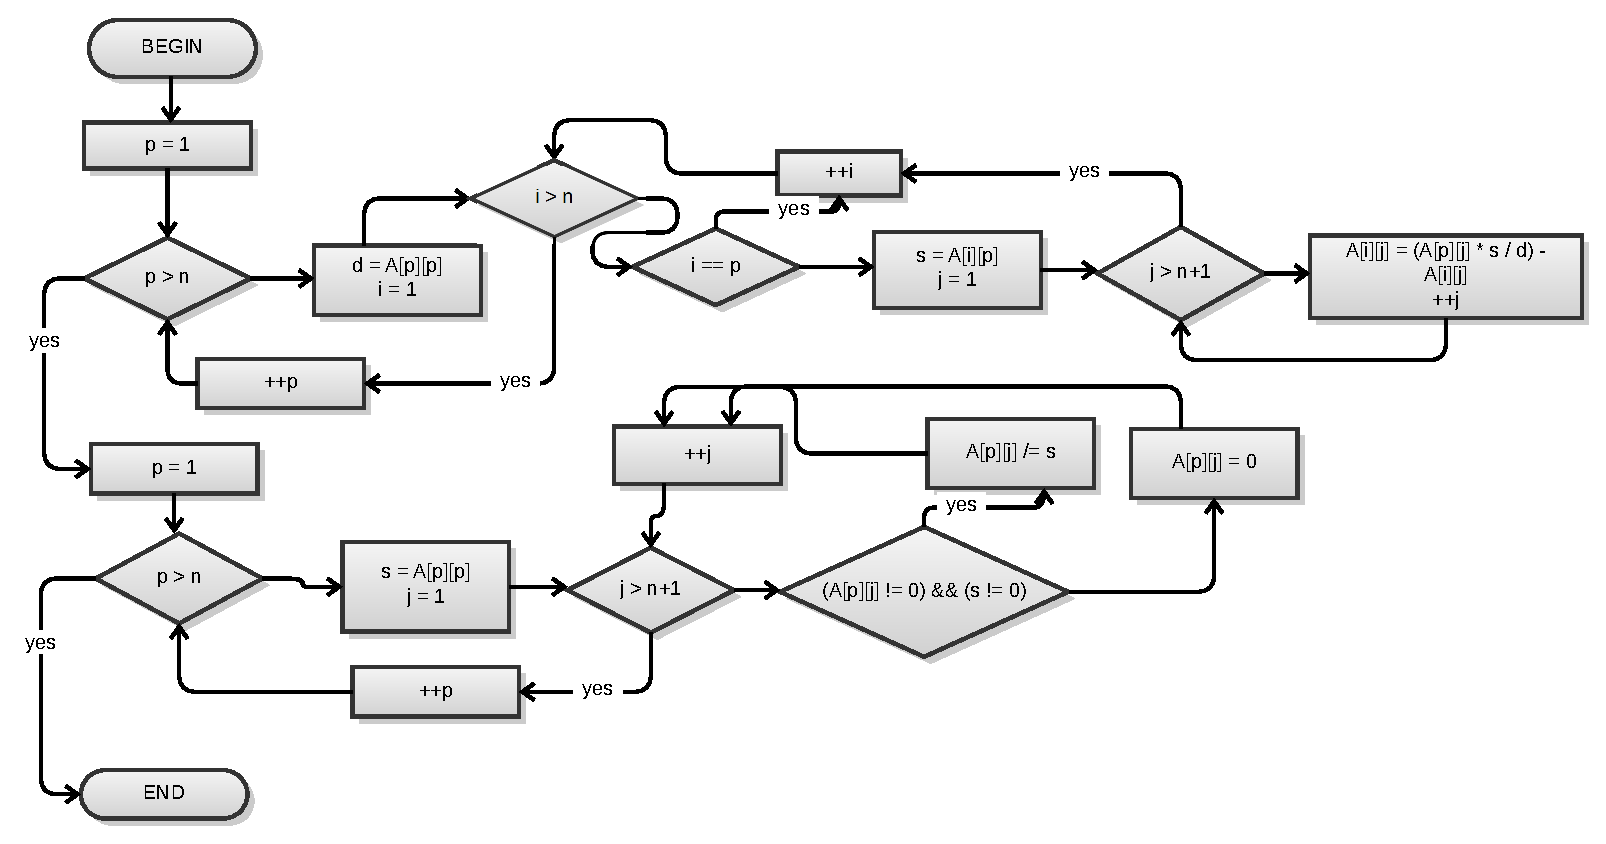
\includegraphics[scale=0.85]{flowchart.eps}
      \end{center}
      \caption{Блок-схема алгоритма}
      \label{fig:flowchart}
    \end{figure}
  \end{landscape}

\section{Выводы}
  В данной лабораторной работе был реализован метод Жордана"=Гаусса решения
  систем линейных алгебраических уравнений.

  Полученное решение было проверено подстановкой в начальное условие
  результата.
  В результате сравнения вектора свободных членов, была получена оценка
  точности~\eqref{eq:delta}
\newpage
\section{Приложения}
  \subsection{Графическая форма приложения}
    \begin{figure}[h]
      \begin{center}
        \includegraphics{screenshot.png}
      \end{center}
      \caption{Графическая форма приложения}
      \label{fig:gui}
    \end{figure}
    \clearpage
  \subsection{Исходные тексты}
    \subsubsection{CMakeLists.txt}
      \lstinputlisting{/home/projects/apps-for-computing/lab1/CMakeLists.txt}
    \subsubsection{lab1\_widget.hxx}
      \lstinputlisting{/home/projects/apps-for-computing/lab1/lab1_widget.hxx}
    \subsubsection{lab1\_widget.cxx}
      \lstinputlisting{/home/projects/apps-for-computing/lab1/lab1_widget.cxx}
\end{document}
